\documentclass[twoside]{article}
\setlength{\oddsidemargin}{0.25 in}
\setlength{\evensidemargin}{-0.25 in}
\setlength{\topmargin}{-0.6 in}
\setlength{\textwidth}{6.5 in}
\setlength{\textheight}{8.5 in}
\setlength{\headsep}{0.75 in}
\setlength{\parindent}{0 in}
\setlength{\parskip}{0.1 in}
\newcommand{\eqdef}{:\mathrel{\mathop=}}
\newcommand{\norm}[1]{\left\lVert #1 \right\rVert}

%
% ADD PACKAGES here:
%

\usepackage{amsmath,amsfonts,graphicx}

%
% The following commands set up the lecnum (lecture number)
% counter and make various numbering schemes work relative
% to the lecture number.
%
\newcounter{lecnum}
\renewcommand{\thepage}{\thelecnum-\arabic{page}}
\renewcommand{\thesection}{\thelecnum.\arabic{section}}
\renewcommand{\theequation}{\thelecnum.\arabic{equation}}
\renewcommand{\thefigure}{\thelecnum.\arabic{figure}}
\renewcommand{\thetable}{\thelecnum.\arabic{table}}
\newcommand{\indep}{\raisebox{0.05em}{\rotatebox[origin=c]{90}{$\models$}}}

%
% The following macro is used to generate the header.
%
\newcommand{\lecture}[4]{
   \pagestyle{myheadings}
   \thispagestyle{plain}
   \newpage
   \setcounter{lecnum}{#1}
   \setcounter{page}{1}
   \noindent
   \begin{center}
   \framebox{
      \vbox{\vspace{2mm}
    \hbox to 6.28in { {\bf Advanced Machine Learning
	\hfill Fall 2020} }
       \vspace{4mm}
       \hbox to 6.28in { {\Large \hfill Lecture #1: #2  \hfill} }
       \vspace{2mm}
       \hbox to 6.28in { {\it  #3 \hfill  #4} }
      \vspace{2mm}}
   }
   \end{center}
   \markboth{Lecture #1: #2}{Lecture #1: #2}

   {\bf Note}: {\it LaTeX template courtesy of UC Berkeley EECS dept.}

   {\bf Disclaimer}: {\it These notes are adapted from ETH's Advanced Machine Learning Course and "Machine Learning: a Probabilistic Perspective" book.}
   \vspace*{4mm}
}
%
% Convention for citations is authors' initials followed by the year.
% For example, to cite a paper by Leighton and Maggs you would type
% \cite{LM89}, and to cite a paper by Strassen you would type \cite{S69}.
% (To avoid bibliography problems, for now we redefine the \cite command.)
% Also commands that create a suitable format for the reference list.
\renewcommand{\cite}[1]{[#1]}
\def\beginrefs{\begin{list}%
        {[\arabic{equation}]}{\usecounter{equation}
         \setlength{\leftmargin}{2.0truecm}\setlength{\labelsep}{0.4truecm}%
         \setlength{\labelwidth}{1.6truecm}}}
\def\endrefs{\end{list}}
\def\bibentry#1{\item[\hbox{[#1]}]}

%Use this command for a figure; it puts a figure in wherever you want it.
%usage: \fig{NUMBER}{SPACE-IN-INCHES}{CAPTION}
\newcommand{\fig}[3]{
			\vspace{#2}
			\begin{center}
			Figure \thelecnum.#1:~#3
			\end{center}
	}
% Use these for theorems, lemmas, proofs, etc.
\newtheorem{theorem}{Theorem}[lecnum]
\newtheorem{lemma}[theorem]{Lemma}
\newtheorem{proposition}[theorem]{Proposition}
\newtheorem{claim}[theorem]{Claim}
\newtheorem{corollary}[theorem]{Corollary}
\newtheorem{definition}[theorem]{Definition}
\newenvironment{proof}{{\bf Proof:}}{\hfill\rule{2mm}{2mm}}

% **** IF YOU WANT TO DEFINE ADDITIONAL MACROS FOR YOURSELF, PUT THEM HERE:

\newcommand\E{\mathbb{E}}

\begin{document}
%FILL IN THE RIGHT INFO.
%\lecture{**LECTURE-NUMBER**}{**DATE**}{**LECTURER**}{**SCRIBE**}
\lecture{11}{Non-parametric Bayesian methods}{}{}
%\footnotetext{These notes are partially based on those of Nigel Mansell.}

% **** YOUR NOTES GO HERE:

% Some general latex examples and examples making use of the
% macros follow.  
%**** IN GENERAL, BE BRIEF. LONG SCRIBE NOTES, NO MATTER HOW WELL WRITTEN,
%**** ARE NEVER READ BY ANYBODY.


\section{Model Selection} % Don't be this informal in your notes!

We start our discussion by modeling the posterior distribution:

\begin{equation*}
\begin{aligned}
   & p(\theta | x) = e^{-\beta w(\theta,x)}
   \\
   & w(\theta,x) = R(\theta,x) - F(x)\\
   & F(x) = - \dfrac{1}{\beta} \log{\int{e^{\beta R(\theta,x)}d\theta}} &&& \text{(Normalization term for $p(\theta|x)$)}
  \end{aligned}
\end{equation*}
 
 Next, we can compute the validation error on training set $x'$ and validation set $x''$:

\begin{equation*}
\begin{aligned}
   & \mathbb{E}_{\theta|x'} \Big[ - \log{p(\theta|x'')}\Big]
   \\
   & = \mathbb{E}_{\theta|x'} \Big[ - \beta w(\theta,x'')\Big]\\
   & = \beta \Big( \underbrace{\mathbb{E}_{\theta|x'} \Big[ R(\theta,x'')\Big]}_{Loss} \underbrace{-F(x'')}_\text{Free Energy} \Big ) &&& \text{(Note that $F(x'')$ does not depend on $\theta$ since we integrate it out)}
  \end{aligned}
\end{equation*}

The problem, in practice, is that people just minimize the loss while completely ignoring the free energy. This is the draw back of using the validation error for model selection.

To overcome this limitation, we can perform  "posterior selection":

\begin{equation*}
\begin{aligned}
   & \underset{p(.|.)}{min} \; \mathbb{E}_{\theta|x'} \Big[ - \log{p(\theta|x'')}\Big] \geq \underset{p(.|.)}{min} \; - \log{\mathbb{E}_{\theta|x'} \Big[ {p(\theta|x'')}}\Big] &&& \text{(Jensen's inequality)}
   \\
   & = \underset{p(.|.)}{min} \; - \log{ \Big( \int{p(\theta|x') p(\theta|x'') d\theta} \Big)} \\
   & = - \underset{p(.|.)}{max} \;  \log{ \Big( \underbrace{\int{p(\theta|x') p(\theta|x'') d\theta}}_{\text{Probability Kernel $k(x',x'')$}} \Big)}
 \end{aligned}
\end{equation*}
\newpage 

A few remarks on this:
\begin{itemize}
    \item The kernel $k(x',x'')$  measures the "agreement" of the two posteriors.
    \item This strategy chooses a posterior that is concentrated (peaked) and agrees between $x'$ and $x''$
    \item When we apply Jensen's inequality we have no guarantee that the posteriors (the one of the original optimization problem and the one from Jensen's) are similar.
    \item Maximizing the $\mathbb{E}_{x',x''} \Big[ \log{k(x',x'')} \Big ]$ is a metric concept, since the kernel captures the similarity between $x'$ and $x''$. Whereas minimizing $\mathbb{E}_{\theta | x'} \Big [R(\theta,x'')\Big]$ is a search strategy based on a partial order. The argument we make here is that the latter is more sensible to noise. (In the space of $\theta$, two solutions might be far away from each other and still have the same cost value)
\end{itemize}


\section{Dirichlet Processes}
The principle problem with finite mixture models is how to choose the number of components $\mathbf{K}$. However, in many cases, there is no well- defined number of clusters. It would be much better if we did not have to choose K at all.
In this section, we discuss infinite mixture models, in which we do not impose any a priori bound on $K$. To do this, we will use a non-parametric prior based on the Dirichlet process ($DP$). This allows the number of clusters to grow as the amount of data increases.

\subsection{Stick-breaking Construction}
To build the mixture model we need to sample the cluster probabilities:  $\rho_{1 : K} \sim Dir(a_{1 :K})$.\\ However, there are two problems:
\begin{itemize}
    \item As $K \to \infty$ we cannot sample infinite points from $Dir()$.
    \item The sum of these probabilities should sum to 1. 
\end{itemize}
We observe that:
$$ \rho_{1:K} \sim Dir\Big(a_{1:K}\Big) \iff
\rho_{1} = Beta\Big(a_{1}, \sum_{k=1}^{K} a_{k} - a_{1} \Big) \; \indep \; Dir\Big(a_{2:K} \Big)
$$

Thus, we can sample from the Dirichlet using this technique:
\begin{figure}[h]
\centering
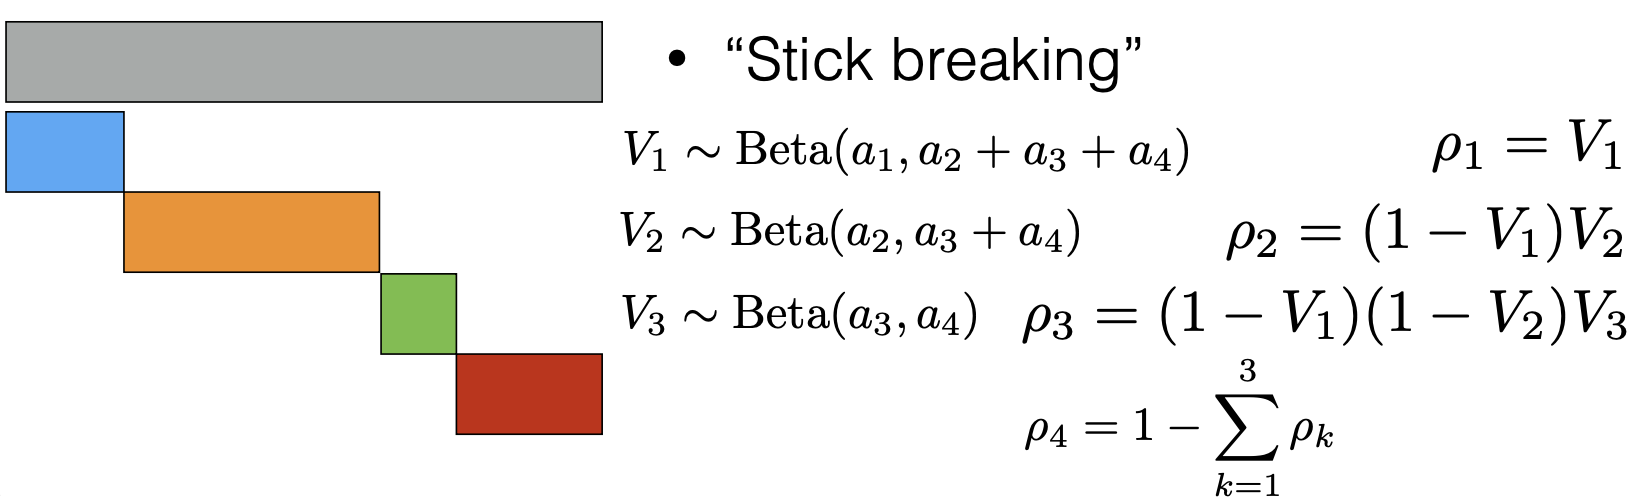
\includegraphics[width=0.7\textwidth]{img/stick-breaking.png}
\end{figure}

\newpage

How can we generate $K \to \infty$ probabilities that strictly sum to one?\\ 
We fix the Betas in the stick-breaking process to $Beta(1,\alpha)$.

\vspace{1mm}

\begin{figure}[h]
\centering
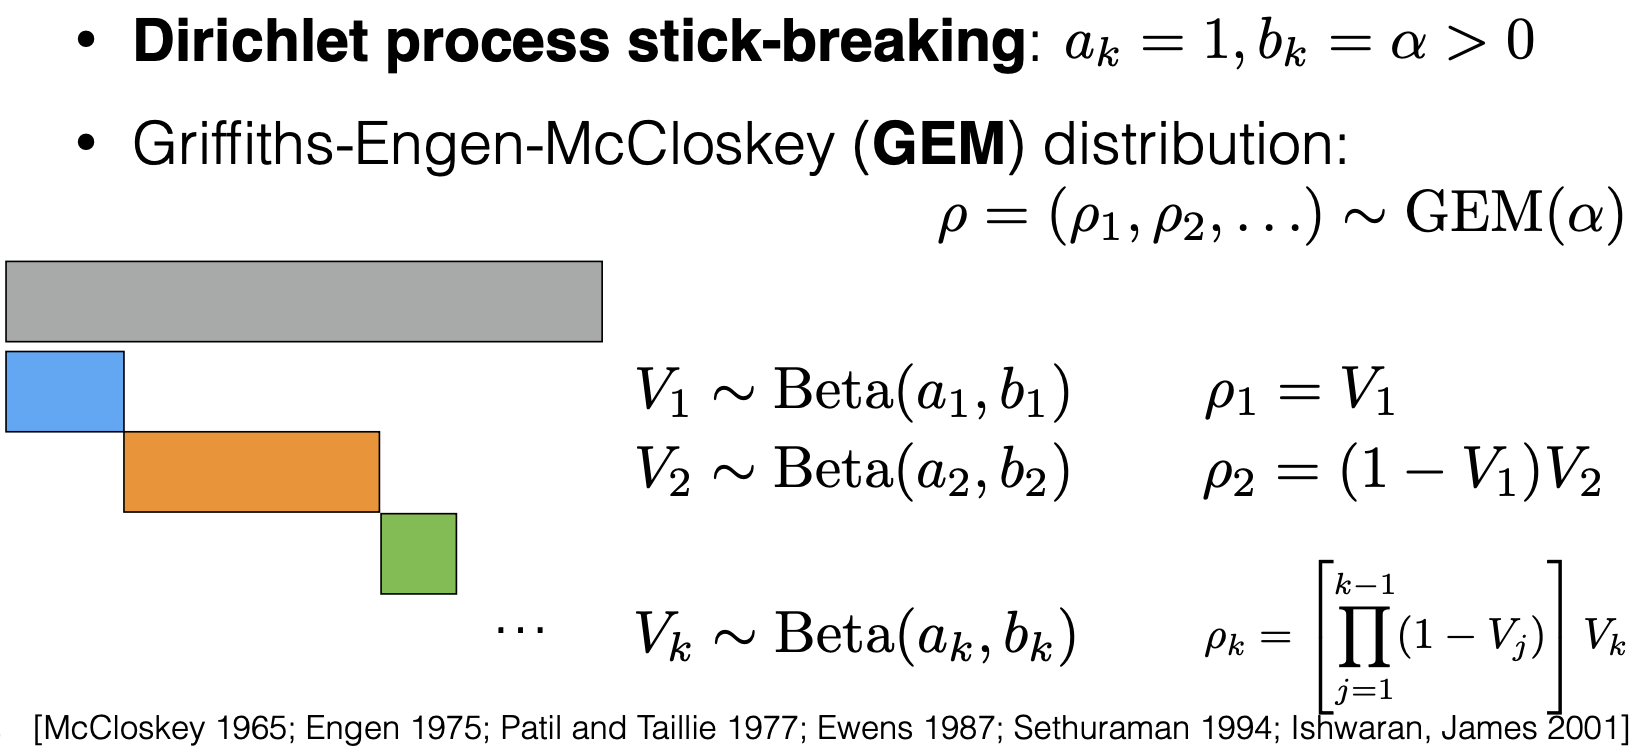
\includegraphics[width=0.7\textwidth]{img/stick-breaking2.png}
\end{figure}

\vspace{1mm}
We finally obtain a distribution $\rho \sim GEM(\alpha)$ from which we can sample our infinite probabilities.
Observe that $\alpha$ is an hyper-parameter that regulates how much stick the first draws will obtain. The larger the $\alpha$ the smaller the first piece of the stick will be.

\begin{figure}[h]
\centering
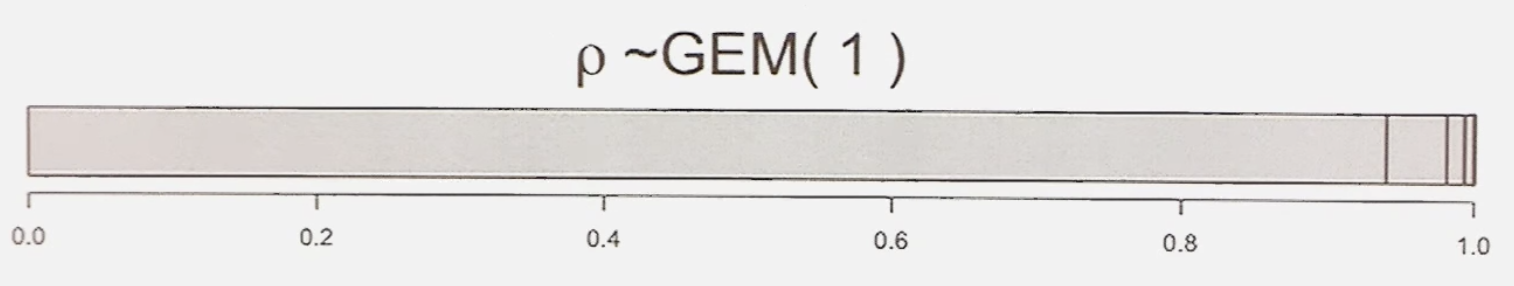
\includegraphics[width=0.6\textwidth]{img/gem1.png}
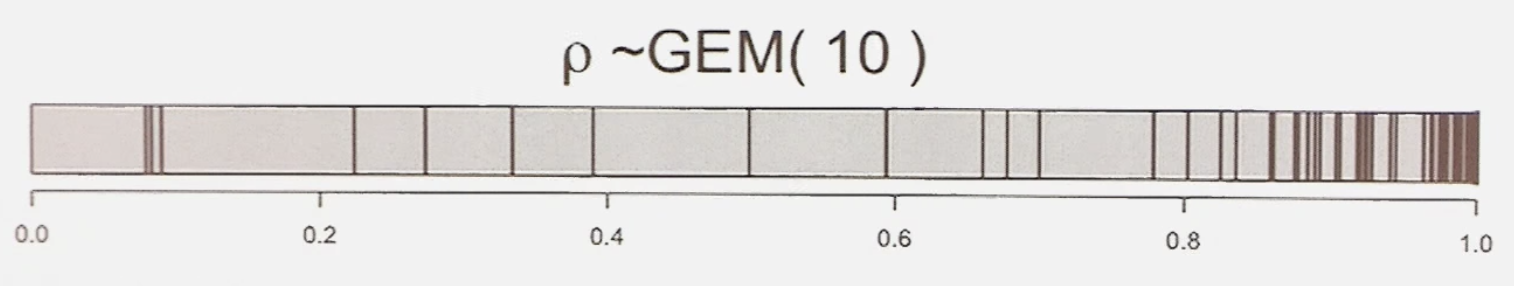
\includegraphics[width=0.6\textwidth]{img/gem10.png}
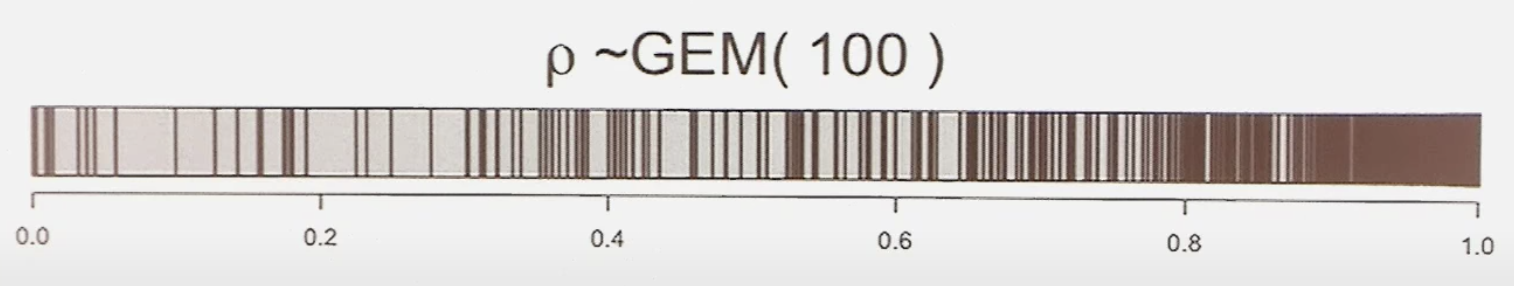
\includegraphics[width=0.6\textwidth]{img/gem100.png}
\end{figure}
\newpage
\subsection{Mixture Model}
We now have all we need to build our Dirichlet Process Mixture Model. \\ \\
First, we draw an infinity of cluster probabilities from $\rho \sim GEM(\alpha)$

\begin{figure}[h]
    \centering
    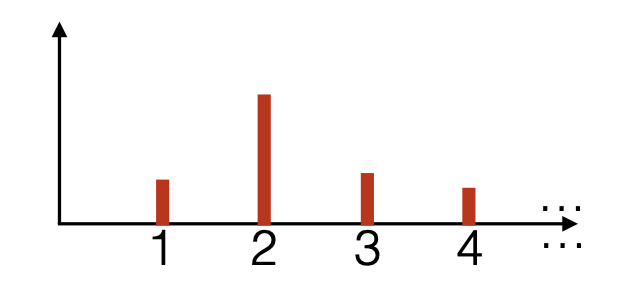
\includegraphics[width=0.3\textwidth]{img/frequencies.png}
\end{figure}

Second, we draw an infinity of $\mu_{k} \sim \mathcal{N}\Big(\mu_{0}, \Sigma_{0}\Big), k=1,2 \ldots$  and we assign each $u_{k}$ to the respective probability $\rho$.

\begin{figure}[h]
    \centering
    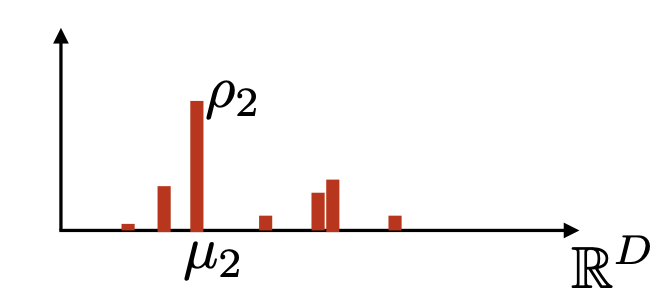
\includegraphics[width=0.3\textwidth]{img/us.png}
\end{figure}

The resulting distribution is $G= \sum_{k=1}^{\infty} \rho_{k} \delta{\mu_{k}} = DP\Big(\alpha, \mathcal{N}(\mu_{0}, \Sigma_{0})\Big)$. We have successfuly constructed a Dirichlet Process. 


To generate data from this model, we can sample $z_{n} \sim Categorical(\rho)$ and $\mu_{n} = \mu_{z_{n}}$  i.e. $\mu_{n} \sim G$. Next, we sample the data point from $x_{n} \sim \mathcal{N}(\mu_{n}, \Sigma_{0})$.

However, this is unfeasible in practice because we need to draw an infinity of $\rho$. The key idea to solve this problem, is to draw the $\rho$ on demand. We can draw from $GEM(2)$ with  Uniform$(0,1)$: if the sample we draw from the uniform distribution (red cursor in figure) is already covered we draw $x_{1}$ from the corresponding Gaussian with mean $\mu_{1}$. If it is not covered (white space in figure) we continue the stick breaking process until it is covered. 


\begin{figure}[h]
    \centering
    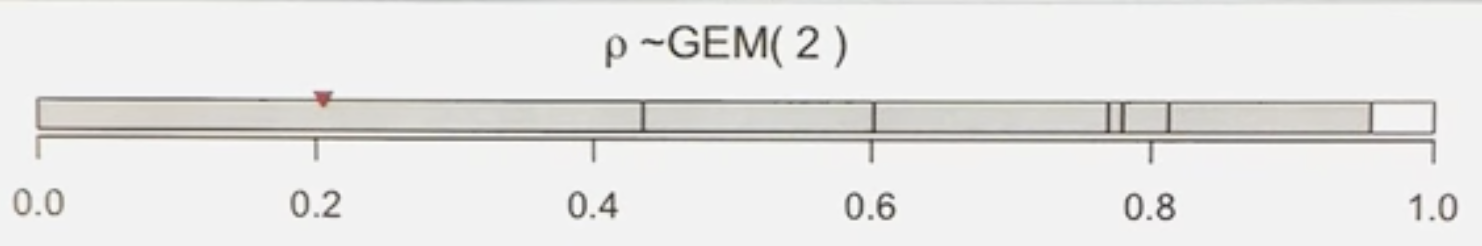
\includegraphics[width=0.6\textwidth]{img/gem2.png}
\end{figure}
\newpage
\subsection{Chinese Restaurant Process}
Chinese restaurant process or CRP, is based on the seemingly infinite supply of tables at certain Chinese restaurants. 
The analogy is as follows: The tables are like clusters, and the customers are like observations. When a person enters the restaurant, he may choose to join an existing table with probability proportional to the number of people already sitting at this table (the $|\tau|$ term); otherwise, with a probability that diminishes as more people enter the room (due to the $\dfrac{1}{\alpha + n} $ term), he may choose to sit at a new table. The result is a distribution over partitions of the integers, which is like a distribution of customers to tables.
The fact that currently occupied tables are more likely to get new customers is sometimes called the \textbf{rich get richer} phenomenon. 

\begin{figure}[h]
    \centering
    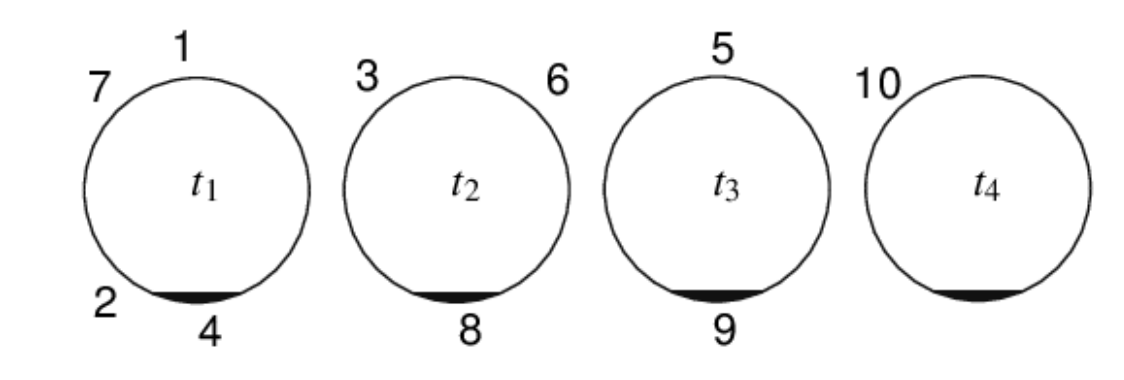
\includegraphics[width=0.6\textwidth]{img/cp.png}
\end{figure}

$$\pi_{[10]} = \{\{1,2,4,7\}, \{3,6,8\},\{5,9\},\{10\}\}$$
\[
  P(\text{customer} \; n+1 \; \text{joins table} \; \tau \; | \pi)=
  \begin{cases}
                                  \dfrac{ |\tau|}{\alpha+n} & \text{if $\tau \in \pi$} \\
                                   \dfrac{\alpha}{\alpha +n} & \text{otherwise} \\
  \end{cases}
\]

The probability for a specific tables configuration is given by:
$$P(\pi_{[n]}) =\dfrac{ \alpha^{|\pi_{[n]}|}}{\alpha^{(n)}} \prod_{\tau \in \pi_{[n]}} (\tau -1)! $$ 
where $\alpha^{(n)}$ is the ascending factorial.

\subsection{Exchangeability}

Let $(X_{1},X_{2},\ldots)$ be a sequence of random variables. The sequence in exchangeable when, for every permutation $\pi$ of $\mathcal{N}$, the random vectors:

$$(X_{1},X_{2},\ldots) \text{ and} \; (X_{\pi(1)}, X_{\pi(2)}, \ldots)$$

have the same distribution.

\begin{theorem}(De Finetti)\\
Let $(X_{1},X_{2},\ldots)$ be an infinitely exchangeable sequence of random variables. Then , $\forall n$:

$$p(X_{1},\ldots,X_{n}) = \int \Big( \prod_{i=1}^{n} p(x_{i}|G)\Big)dP(G)$$

for some random variable G.

\end{theorem}

In the case of i.i.d. random variables we would only have  one $G$ and the theorem would reduce to $p(X_{1},\ldots,X_{n}) =  \prod_{i=1}^{n} p(x_{i})$
\\ \\
Notice that CRP is exchangeable $\implies $ we can apply De Finetti's Theorem. In the CRP's case, the Dirichlet Process is the random variable G of De Finetti's theorem. The intuition behind this is that the probability of a particular table configuration is given by a "voting"  weighted on all the underlying distributions G from which the probabilities of the tables (remember the $\rho$'s) are picked from.

\subsection{Fitting}
We can leverage exchangeability to fit our model: any point can be considered the last arrived.\\ Considering the case of CRP: for	each	observation, we	remove	the	customer dish from	the	restaurant	and	resample	as	if	they	were	the	last	to	enter.

\begin{itemize}
    \item Take a random guess initially.
    \item Unassign observation i.
    \item Compute $p(z_{i} | z_{-i}, x, \alpha, \mu)$ which  represents the cluster assignment for element i.
    \item Update $z_{i}$ by sampling from this distribution.
    \item Keep going.
    
\end{itemize}

$p(z_{i} | z_{-i}, x, \alpha, \mu)$ is computed as follows:

$$p(z_{i}=k | z_{-i}, \mathbf{x}, \alpha, \mathbf{\mu}) \propto \underbrace{p(z_{i}=k | z_{-i}, \alpha)}_{Prior} \; \underbrace{p(x_{i}| \mu, z_{i}=k, z_{-i}, \mathbf{x_{-i}})}_{Likelihood} \;$$


The prior computation is simple (CRP):


\[
  p(z_{i}=k | z_{-i}, \alpha)=
  \begin{cases}
                                  \dfrac{N_{k,-i}}{\alpha+N-1} & \text{for existing k} \\
                                   \dfrac{\alpha}{\alpha +N-1} & \text{otherwise} \\
  \end{cases}
\]

Finally, for the likelihood we don't need to consider point in $x$ that are not in cluster $k$:

\[
  p(x_{i}| \mu, z_{i}=k, z_{-i}, \mathbf{x_{-i}})=
  \begin{cases}
                                  p(x_{i} | x_{-i,k}, \mu) & \text{for existing k} \\
                                   p(x_{i} | \mu) & \text{otherwise} \\
  \end{cases}
\]




\end{document}